% Options for packages loaded elsewhere
\PassOptionsToPackage{unicode}{hyperref}
\PassOptionsToPackage{hyphens}{url}
%
\documentclass[
]{article}
\usepackage{amsmath,amssymb}
\usepackage{lmodern}
\usepackage{iftex}
\ifPDFTeX
  \usepackage[T1]{fontenc}
  \usepackage[utf8]{inputenc}
  \usepackage{textcomp} % provide euro and other symbols
\else % if luatex or xetex
  \usepackage{unicode-math}
  \defaultfontfeatures{Scale=MatchLowercase}
  \defaultfontfeatures[\rmfamily]{Ligatures=TeX,Scale=1}
\fi
% Use upquote if available, for straight quotes in verbatim environments
\IfFileExists{upquote.sty}{\usepackage{upquote}}{}
\IfFileExists{microtype.sty}{% use microtype if available
  \usepackage[]{microtype}
  \UseMicrotypeSet[protrusion]{basicmath} % disable protrusion for tt fonts
}{}
\makeatletter
\@ifundefined{KOMAClassName}{% if non-KOMA class
  \IfFileExists{parskip.sty}{%
    \usepackage{parskip}
  }{% else
    \setlength{\parindent}{0pt}
    \setlength{\parskip}{6pt plus 2pt minus 1pt}}
}{% if KOMA class
  \KOMAoptions{parskip=half}}
\makeatother
\usepackage{xcolor}
\usepackage[left=2cm,right=2cm,top=1.5cm,bottom=1.5cm]{geometry}
\usepackage{graphicx}
\makeatletter
\def\maxwidth{\ifdim\Gin@nat@width>\linewidth\linewidth\else\Gin@nat@width\fi}
\def\maxheight{\ifdim\Gin@nat@height>\textheight\textheight\else\Gin@nat@height\fi}
\makeatother
% Scale images if necessary, so that they will not overflow the page
% margins by default, and it is still possible to overwrite the defaults
% using explicit options in \includegraphics[width, height, ...]{}
\setkeys{Gin}{width=\maxwidth,height=\maxheight,keepaspectratio}
% Set default figure placement to htbp
\makeatletter
\def\fps@figure{htbp}
\makeatother
\setlength{\emergencystretch}{3em} % prevent overfull lines
\providecommand{\tightlist}{%
  \setlength{\itemsep}{0pt}\setlength{\parskip}{0pt}}
\setcounter{secnumdepth}{-\maxdimen} % remove section numbering
\ifLuaTeX
  \usepackage{selnolig}  % disable illegal ligatures
\fi
\IfFileExists{bookmark.sty}{\usepackage{bookmark}}{\usepackage{hyperref}}
\IfFileExists{xurl.sty}{\usepackage{xurl}}{} % add URL line breaks if available
\urlstyle{same} % disable monospaced font for URLs
\hypersetup{
  pdftitle={Stats 15 - Homework 1},
  pdfauthor={Your Name Here},
  hidelinks,
  pdfcreator={LaTeX via pandoc}}

\title{Stats 15 - Homework 1}
\author{Your Name Here}
\date{}

\begin{document}
\maketitle

Homework text and questions: Copyright Miles Chen. Do not post, share,
or distribute without permission.

\hypertarget{academic-integrity-statement}{%
\section{Academic Integrity
Statement}\label{academic-integrity-statement}}

By modifying this statement , I, \textbf{Your Name Here}, declare that
all of the work in this assignment is my own original work. At no time
did I look at the code of other students nor did I search for code
solutions online. I understand that plagiarism on any single part of
this assignment will result in a 0 for the entire assignment and that I
will be referred to the dean of students.

\hypertarget{part-1-textbook-chapter-2-exercise-3}{%
\section{Part 1: Textbook Chapter 2, Exercise
3}\label{part-1-textbook-chapter-2-exercise-3}}

\hypertarget{example-of-a-compelling-graphic-display}{%
\subsection{Example of a compelling graphic
display}\label{example-of-a-compelling-graphic-display}}

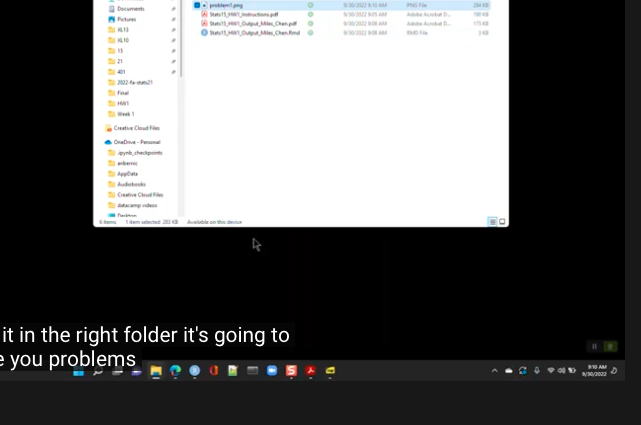
\includegraphics[height=3in]{problem1}

Replace the following text with your response:

This image was taken from:
\url{https://www.latimes.com/projects/california-coronavirus-cases-tracking-outbreak/}

Aspects that work well:

\begin{itemize}
\tightlist
\item
  reason 1
\item
  reason 2
\end{itemize}

\hypertarget{example-of-a-graphic-display-that-is-less-compelling}{%
\subsection{Example of a graphic display that is less
compelling}\label{example-of-a-graphic-display-that-is-less-compelling}}

Replace this text. Insert a code chunk that will include the graphic.

\hypertarget{part-2-textbook-chapter-2-exercise-6}{%
\section{Part 2: Textbook Chapter 2, Exercise
6}\label{part-2-textbook-chapter-2-exercise-6}}

\begin{itemize}
\tightlist
\item
  What quantity is being shown on the y-axis of each plot?

  \begin{itemize}
  \tightlist
  \item
    Write your response
  \end{itemize}
\item
  List the variables displayed in the data graphic, along with the units
  and a few typical values for each.

  \begin{itemize}
  \tightlist
  \item
    Write your response
  \end{itemize}
\item
  List the visual cues used in the data graphic and explain how each
  visual cue is linked to each variable.

  \begin{itemize}
  \tightlist
  \item
    Write your response
  \end{itemize}
\item
  Examine the graphic carefully. Describe, in words, what information
  you think the data graphic conveys. Do not just summarize the
  data---interpret the data in the context of the problem and tell us
  what it means. (Note: information is meaningful to human beings---it
  is not the same thing as data.)

  \begin{itemize}
  \tightlist
  \item
    Write your response
  \end{itemize}
\end{itemize}

\hypertarget{part-3-textbook-chapter-3-exercise-1}{%
\section{Part 3: Textbook Chapter 3, Exercise
1}\label{part-3-textbook-chapter-3-exercise-1}}

Follow the instructions in the instruction file.

\hypertarget{part-4-textbook-chapter-3-exercise-2}{%
\section{Part 4: Textbook Chapter 3, Exercise
2}\label{part-4-textbook-chapter-3-exercise-2}}

Follow the instructions in the instruction file.

\hypertarget{part-5-textbook-chapter-3-exercise-6}{%
\section{Part 5: Textbook Chapter 3, Exercise
6}\label{part-5-textbook-chapter-3-exercise-6}}

Follow the instructions in the instruction file.

\hypertarget{part-6-textbook-chapter-3-exercise-7}{%
\section{Part 6: Textbook Chapter 3, Exercise
7}\label{part-6-textbook-chapter-3-exercise-7}}

Follow the instructions in the instruction file.

\end{document}
